%% ============================================================================
%%  Physical Review B
%%  Interaction-induced d_{xy} pairing in the checkerboard Hubbard model
%%
%%  Generated by code/build_manuscripts.py. Every number traces to a file in the
%%  repository; pointers are given in comments beside each claim.
%%  TODO before submission: author list, affiliations, acknowledgments, and the
%%  full bibliographic entry marked INCOMPLETE.
%% ============================================================================
\documentclass[aps,prb,reprint,superscriptaddress,amsmath,amssymb,floatfix]{revtex4-2}

\usepackage{graphicx}
\usepackage{bm}
\graphicspath{{../figures/}}

\begin{document}

\title{Interaction-induced $d_{xy}$ pairing in the checkerboard Hubbard model}

% TODO: author list and affiliations to be completed by the authors.
\author{[Author One]}
\affiliation{[Affiliation]}
\author{[Author Two]}
\affiliation{[Affiliation]}

\date{\today}

\begin{abstract}
We study pairing in the half-filled Hubbard model on the checkerboard
lattice by constrained-path quantum Monte Carlo. Separating the
interaction-induced vertex from the uncorrelated part of the pair-field
correlator, we find that the vertex vanishes identically in the noninteracting
limit in all four channels examined, so any pairing tendency is generated by the
interaction rather than inherited from the band structure. The $d_{xy}$ vertex is
the largest of the four above a crossover anisotropy $\delta_c$ and grows
monotonically with interaction strength, from $3.347(8)$ at $U = 2$ to
$5.952(22)$ at $U = 4.5$, peaking at $\delta = 0.4$ in both cases. The crossover
is nearly independent of interaction strength and becomes more so with system
size, its spread falling from $0.148$ to $0.028$ between $8\times8$ and
$12\times12$ lattices while the mean moves from $0.235$ to $0.192$, which
identifies $\delta_c \approx 0.19$ as a property of the lattice geometry. The
$d_{xy}$ vertex grows by a factor between $2.18$ and $2.38$ over the same range
of sizes, while the $d_{x^2-y^2}$ vertex remains positive everywhere and never
becomes repulsive. The dominant channel lies outside the basis used in earlier
finite-temperature work on a related checkerboard Hamiltonian.
\end{abstract}

\maketitle

% ---------------------------------------------------------------------------
\section{Introduction}
% ---------------------------------------------------------------------------

Altermagnets combine a vanishing net moment with a spin-split band structure, a
combination long assumed to require either ferromagnetism or spin-orbit
coupling~\cite{Smejkal2022a,Smejkal2022b,SmejkalCrystal,Mazin2021}. The symmetry
classification and the order-parameter description have since been put on a
group-theoretic footing~\cite{McClarty2024,Bhowal2024,Roig2024}, and the state has
been identified in MnTe~\cite{Krempasky2024,Lee2024,Hariki2025},
CrSb~\cite{Reimers2024}, and RuO$_2$~\cite{Feng2022,Fedchenko2024}, though the last
of these remains contested~\cite{Bai2024}. Proposals for altermagnetic
superconductivity have followed~\cite{Brekke2023,Ouassou2023,Zhu2023,Chakraborty2024}.
The splitting follows from the crystal
symmetry. The two opposite-spin sublattices are connected by a rotation rather
than by a translation or an inversion, so the spin degeneracy that a conventional
antiferromagnet enforces is absent.

Most microscopic models of this state build the splitting into the Hamiltonian,
usually through a spin-dependent hopping. The splitting is then present already
at zero interaction, and the question of whether interactions alone can produce
it is left open~\cite{Leeb2024}. The Lieb lattice, whose flat band makes the
interacting problem sharp~\cite{Lieb1989,Mielke1991,Tasaki1992}, has been studied
twice for this purpose, and both papers state the gap directly,
noting that unbiased studies establishing an altermagnet as the ground state of
an interacting Hamiltonian are lacking~\cite{Kaushal2025,Duerrnagel2025}. Both
use methods with a controlled range of validity, unrestricted Hartree-Fock with
exact diagonalization on small clusters in the first case and a functional
renormalization group treatment of the weak-coupling limit in the second.

The checkerboard lattice offers a route to the same physics without putting it in
by hand. It is a square lattice with diagonal bonds on alternating plaquettes, so
the two sublattices are exchanged by a fourfold rotation about a plaquette center
but by no translation. The hopping is spin independent and the interaction is a
uniform on-site Hubbard $U$. Any spin splitting therefore appears only once
magnetic correlations develop, which is the emergent route rather than the
built-in one.

Here we ask what the interaction does to pairing on this lattice, independently
of whether long-range magnetic order develops. We report constrained-path
quantum Monte Carlo calculations of the pair-field vertex in four channels at
half filling on lattices of $8\times8$, $10\times10$, and $12\times12$ sites. The
vertex is zero at $U = 0$ in every channel, the $d_{xy}$ channel leads above a
crossover anisotropy that converges with system size, and the $d_{xy}$ vertex
grows with system size at every interaction strength studied.

% ---------------------------------------------------------------------------
\section{Model and method}
\label{sec:model}
% ---------------------------------------------------------------------------

We consider the single-band Hubbard model~\cite{Hubbard1963,Arovas2022},
\begin{equation}
H = \sum_{ij\sigma} t_{ij}\, c^{\dagger}_{i\sigma} c^{\phantom{\dagger}}_{j\sigma}
    + U \sum_i n_{i\uparrow} n_{i\downarrow},
\label{eq:H}
\end{equation}
with nearest-neighbor hopping $t_{ij} = t_0$ and diagonal hopping $t_1 + t_2$
along $(1,1)$ and $t_1 - t_2$ along $(1,-1)$ on one sublattice, the two exchanged
on the other. Energies are in units of $|t_0|$, and we set $t_0 = -1$ and
$t_1 = 0.3$ throughout. The anisotropy is parametrized by $\delta$ through
$t_2 = -\delta$, so that $\delta = 0$ restores the plain square lattice with
uniform second-neighbor hopping and the two sublattices become equivalent. All
calculations reported here are at half filling unless stated otherwise.

\begin{figure}[t]
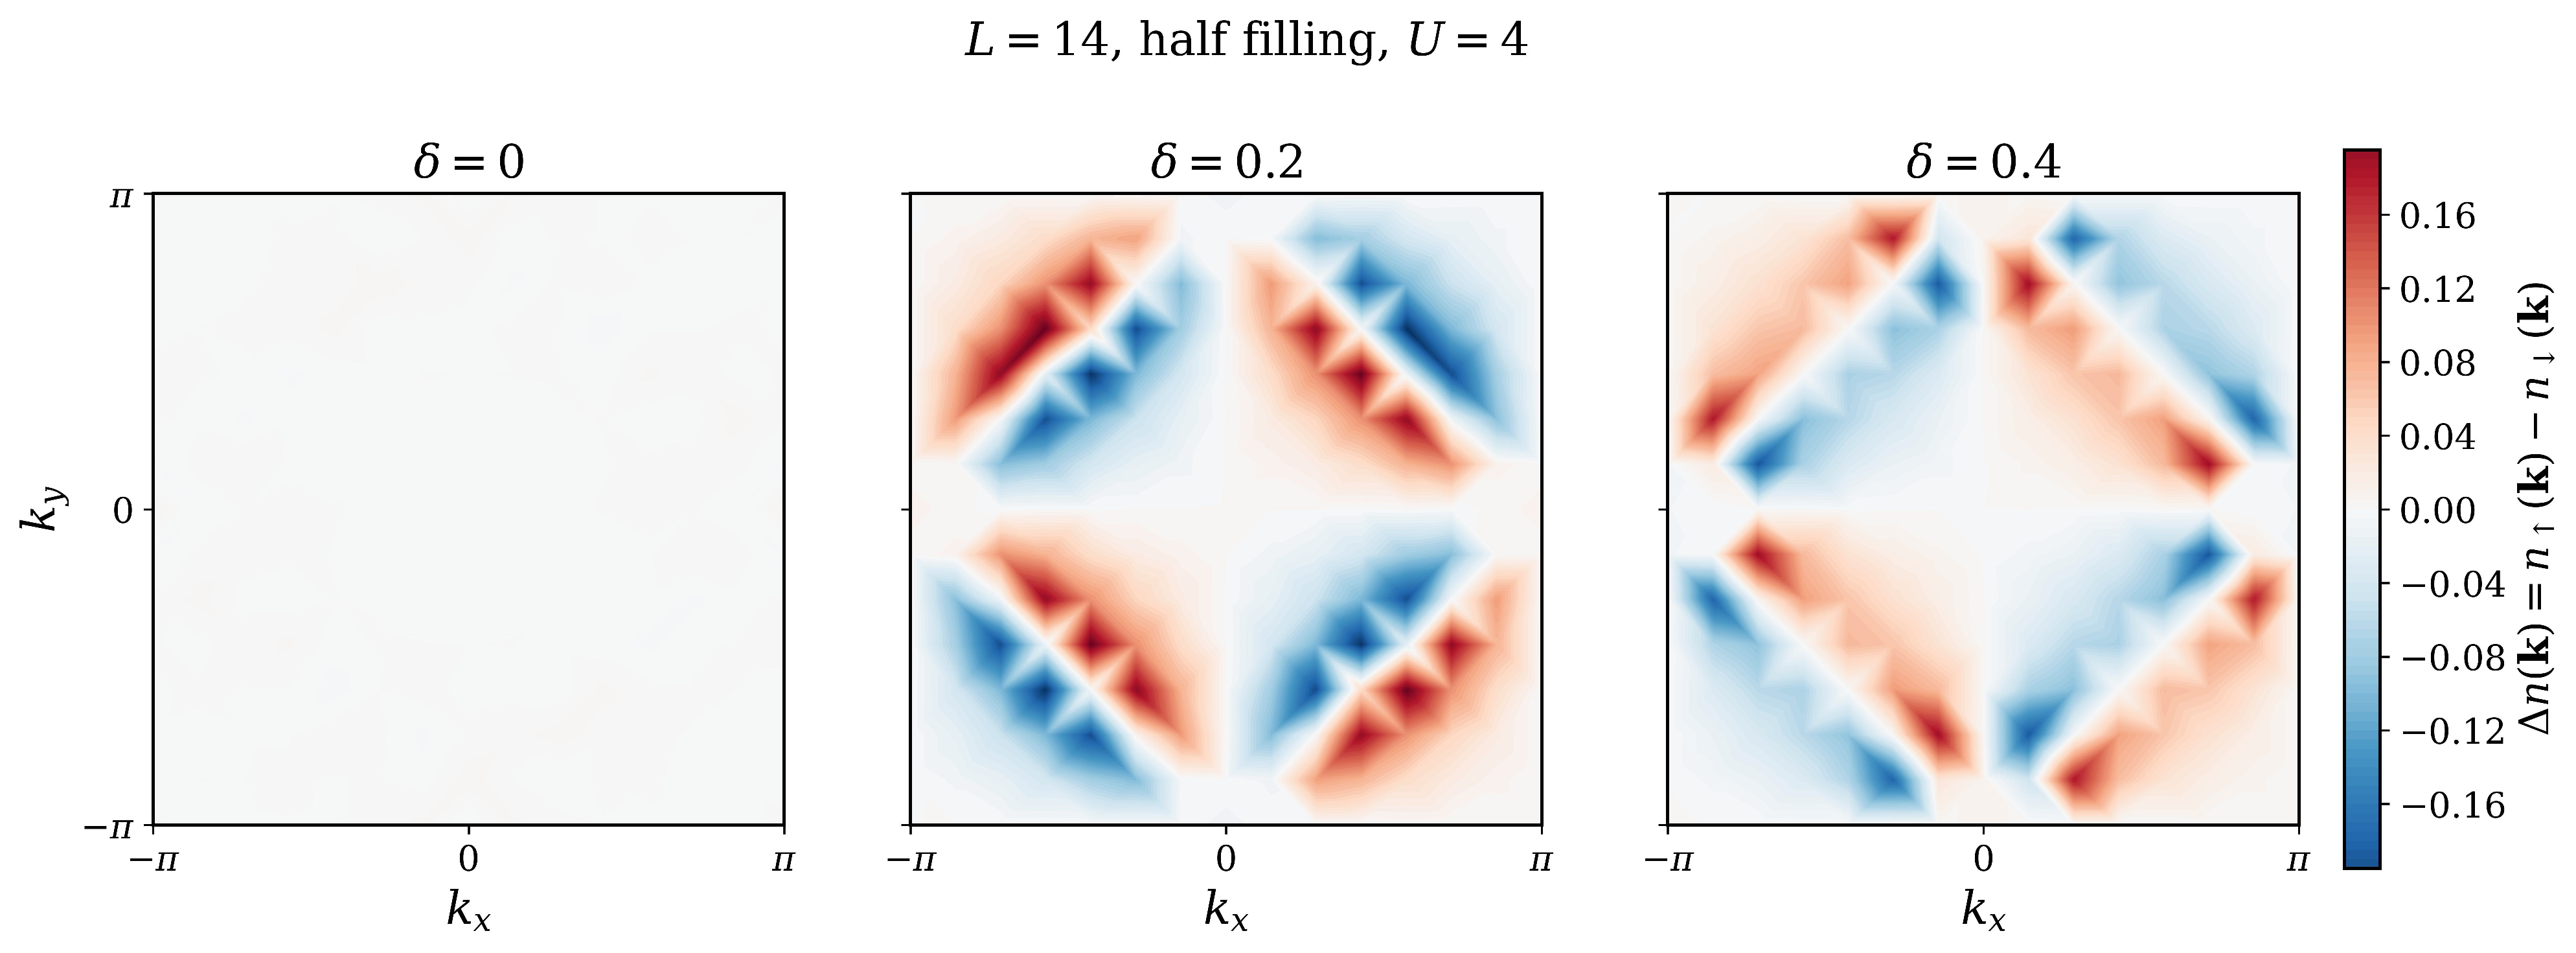
\includegraphics[width=\columnwidth]{1_dnk.pdf}
\caption{Checkerboard lattice and the mean-field spin polarization. The
nearest-neighbor hopping is $t$ and the diagonal hopping is $t_1 \pm \delta$ on
alternating plaquettes, with both spins seeing the same hopping. The momentum
distribution difference $\Delta n(\bm{k})$ vanishes at $\delta = 0$ and develops a
$d_{xy}$ pattern that grows with $\delta$ once a moment forms.}
\label{fig:model}
\end{figure}

The hopping in Eq.~(\ref{eq:H}) is spin independent by construction, so
$n_{\uparrow}(\bm{k}) = n_{\downarrow}(\bm{k})$ at $U = 0$ for every $\delta$.
Figure~\ref{fig:model} shows the geometry together with the mean-field
polarization it produces.

We use constrained-path quantum Monte Carlo
(CPQMC)~\cite{Zhang1997,ZhangKrakauer2003}, an auxiliary-field method~\cite{BSS1981,Hirsch1983,Sorella1989}
in which the constraint removes the exponential sign
problem~\cite{Loh1990,Troyer2005} at the cost of a bias. Benchmarks of the same
method against exact results for the square-lattice Hubbard model are
available~\cite{Hirsch1985,Varney2009,LeBlanc2015,Qin2016}. We use a Trotter step
$\Delta\tau = 0.01$, a projection length $\beta = 32$, and $N_w = 1000$ walkers.
The constrained-path approximation introduces a bias controlled by the trial wave
function, so we do not describe these results as exact. Appendix~\ref{app:trial}
sets out how the trial is chosen, which is not a neutral detail. Doubling the
projection length from $\beta = 32$ to $\beta = 48$ changes the order parameter by
between $0.1\%$ and $4.1\%$ with no systematic drift, which we take as
convergence in $\beta$.
% beta convergence: 32 -> 48 changes 0.1, 1.5, 2.4, 4.1 percent

\begin{figure}[t]
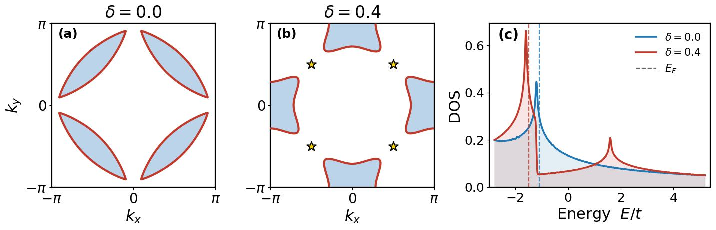
\includegraphics[width=\columnwidth]{2_vhs_dos.pdf}
\caption{Fermi surface and density of states of Eq.~(\ref{eq:H}) at $U = 0$. The
anisotropy $\delta$ moves the van Hove points to incommensurate momenta near the
Fermi level, which is the single-particle change that the interacting
calculations build on.}
\label{fig:vhs}
\end{figure}

% ---------------------------------------------------------------------------
\section{Pairing in the $d_{xy}$ channel}
\label{sec:pairing}
% ---------------------------------------------------------------------------

We compute the pair-field susceptibility in four channels, on-site $s$, extended
$s$, $d_{x^2-y^2}$, and $d_{xy}$, and separate the interaction-induced vertex
from the uncorrelated part. The vertex is the meaningful measure of whether the
interaction builds pairing, since the full correlator is large and positive
already for free electrons. The same separation underlies the long-running
question of whether the plain square-lattice Hubbard model superconducts at
all~\cite{Scalapino2012,Qin2020,Simkovic2024,Huang2019,Jiang2021}, and the study
of pairing driven by repulsion on other lattice
geometries~\cite{Nandkishore2012,Kiesel2012}. Figure~\ref{fig:eqvertex} contrasts
the two.

\begin{figure}[t]
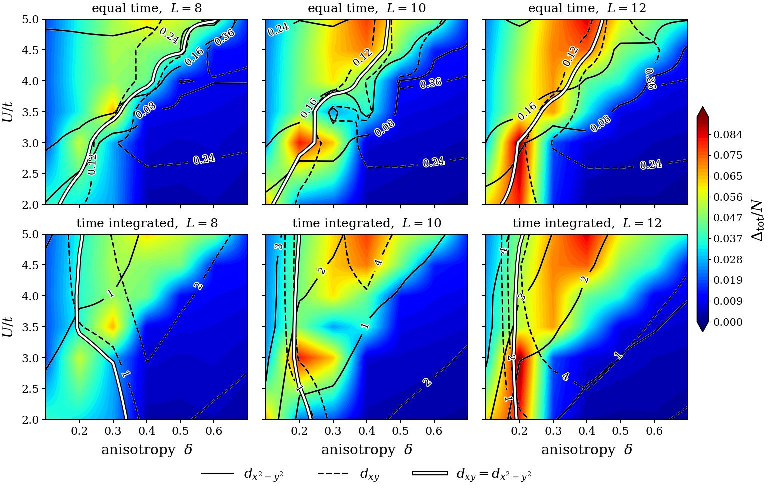
\includegraphics[width=\columnwidth]{fig_2row_eqtime_vertex_3L.pdf}
\caption{Equal-time correlator (top row) against the interaction-induced vertex
(bottom row) for $L = 8$, $10$, and $12$. The channel crossover straightens along
the vertex row, which is why the vertex rather than the full correlator is used
throughout.}
\label{fig:eqvertex}
\end{figure}

Three features stand out. The vertex is zero in all four channels at $U = 0$, so
everything that follows is interaction generated. The on-site $s$ vertex is
negative throughout, as a repulsive $U$ requires. The $d_{xy}$ vertex is the
largest of the four for $\delta \geq 0.3$ at every $U$ studied, and it grows
monotonically with $U$, from $3.347(8)$ at $U = 2$ to $5.952(22)$ at $U = 4.5$,
in both cases peaking at $\delta = 0.4$.
% data/chi_vertex_summary_3L.csv

The leading channel changes with anisotropy. For $\delta \leq 0.2$ the extended
$s$ channel is largest and for $\delta \geq 0.3$ the $d_{xy}$ channel is.
Figure~\ref{fig:ddiff} shows the difference between the two $d$ channels directly
across three sizes.

\begin{figure}[t]
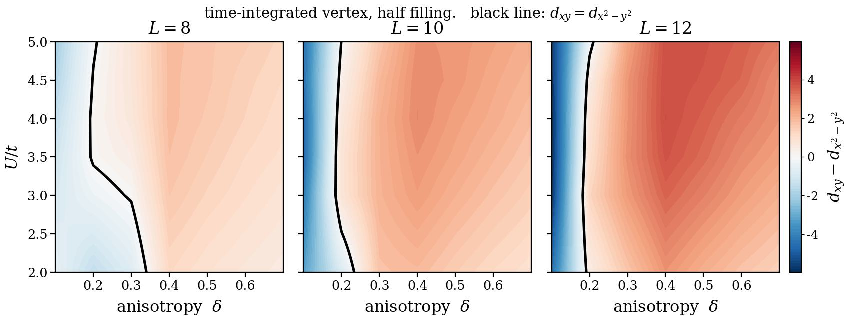
\includegraphics[width=\columnwidth]{fig_ddiff_vertex_3L.pdf}
\caption{Difference between the $d_{xy}$ and $d_{x^2-y^2}$ vertices over the
$(U,\delta)$ plane at $L = 8$, $10$, and $12$. The white contour marks where the
two are equal. $d_{xy}$ leads everywhere to its right, and the boundary moves
very little with size.}
\label{fig:ddiff}
\end{figure}

% ---------------------------------------------------------------------------
\section{Size dependence of the pairing vertex}
\label{sec:vertexfss}
% ---------------------------------------------------------------------------

The vertex was computed at $L = 8$, $10$, and $12$ under identical settings,
which allows the anisotropy of the channel crossover to be followed with size.

The crossover anisotropy $\delta_c$, defined as the value at which the $d_{xy}$
vertex overtakes the extended $s$ vertex, is nearly independent of $U$ and
becomes more so as the lattice grows. Its spread across the six interaction
strengths studied is $0.148$ at $L = 8$, $0.049$ at $L = 10$, and $0.028$ at
$L = 12$, and the mean value moves from $0.235$ to $0.197$ to $0.192$. A
crossover set by the interaction strength would not converge in this way, so we
read $\delta_c \approx 0.19$ as a property of the lattice geometry.
% code/check_vertex_fss.py

The $d_{xy}$ vertex grows with system size at every interaction strength, by a
factor between $2.18$ and $2.38$ from $L = 8$ to $L = 12$. The $d_{x^2-y^2}$
vertex is positive in all $126$ cells at all three sizes, so that channel is
never repulsive even where it is subdominant. The optimal anisotropy for $d_{xy}$
is $\delta = 0.4$ at essentially every size and interaction strength.
Figure~\ref{fig:pairfss} collects these three statements.

\begin{figure}[t]
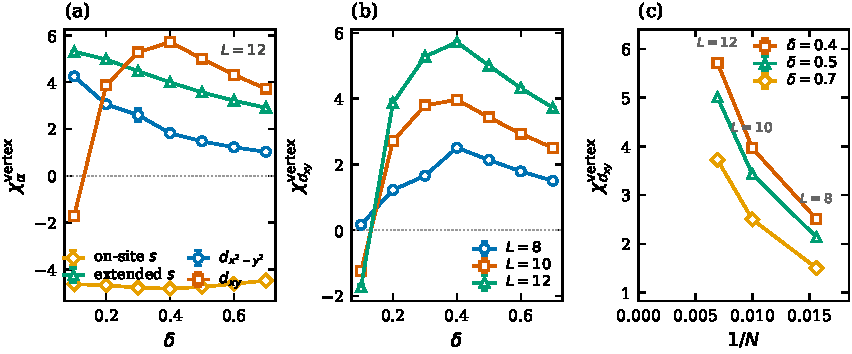
\includegraphics[width=\columnwidth]{fig09_pairing_fss.pdf}
\caption{Interaction-induced pairing vertex at half filling, $U = 4$. (a) The
four channels against $\delta$ at $L = 12$. (b) The $d_{xy}$ vertex against
$\delta$ for three sizes. (c) The $d_{xy}$ vertex against $1/N$ at three
anisotropies, growing with system size in every case.}
\label{fig:pairfss}
\end{figure}

% ---------------------------------------------------------------------------
\section{Robustness and comparison}
\label{sec:robust}
% ---------------------------------------------------------------------------

At half filling with periodic boundaries the noninteracting spectrum of
Eq.~(\ref{eq:H}) is gapless at every $L$ and $\delta$ we examined, so the
occupied set is fixed by the trial state rather than by the spectrum.
Appendix~\ref{app:bc} reports a repeat with antiperiodic boundaries, which shift
the momentum mesh off the high-symmetry points and open a gap. The check is made
on the momentum-space spin polarization $\Delta_{\mathrm{tot}}$ of
Ref.~\cite{OurPRB}, which responds to the mesh more sharply than the pairing
vertex does. The two boundary conditions agree on the sign of
$\partial \Delta_{\mathrm{tot}} / \partial U$ at $\delta = 0.1$ and
$\delta = 0.5$ and disagree at $\delta = 0.3$, which we read as the anisotropy
where the slope passes through zero.

The closest published work is a determinant quantum Monte Carlo study of the
checkerboard Hubbard model that reports $d$-wave and $d + is$ pairing as the
dominant channels~\cite{Pan2024}. The two Hamiltonians are not the same. That
model keeps one diagonal per sublattice and omits the other, whereas
Eq.~(\ref{eq:H}) keeps both, and the two coincide only where our second diagonal
vanishes, at $\delta = t_1 = 0.3$. We verified that the single-particle spectra
agree there to within $4\times10^{-15}$.

At that point, and at half filling, we evaluated the vertex in the basis of
Ref.~\cite{Pan2024} alongside our own. Within their basis the $s$-wave channel is
the larger of the two at $U = 3$, $4$, and $4.5$. Including $d_{xy}$, which their
basis does not contain, gives a $d_{xy}$ vertex larger than either.
% data/pan, analyze_pan.py
The comparison is restricted, since Ref.~\cite{Pan2024} works at density
$n = 0.9$ and temperature $T/t = 1/6$ while our calculations are at half filling
in the ground state, and under the particle-hole transformation that relates the
two signs of the second-neighbor hopping their density maps to $n = 1.1$. The
statement is that the dominant channel we find lies outside the basis used there,
not that the two calculations disagree.

% ---------------------------------------------------------------------------
\section{Conclusion}
% ---------------------------------------------------------------------------

The interaction-induced pairing vertex of the half-filled checkerboard Hubbard
model vanishes at $U = 0$ in all four channels examined and is largest in the
$d_{xy}$ channel above a crossover anisotropy $\delta_c \approx 0.19$. The
crossover is set by the lattice rather than by the interaction, since its spread
across interaction strength falls by a factor of five between $8\times8$ and
$12\times12$ lattices while its mean barely moves. The $d_{xy}$ vertex grows with
system size at every interaction strength, and the $d_{x^2-y^2}$ vertex, while
subdominant, is never repulsive.

The dominant channel is one that earlier finite-temperature work on a related
checkerboard Hamiltonian did not include in its basis. Whether the vertex
develops into a true pairing instability is not settled by the sizes reached
here, and the constrained-path bias remains.

\appendix

% ---------------------------------------------------------------------------
\section{Trial wave function and the selection of the constrained path}
\label{app:trial}
% ---------------------------------------------------------------------------

The constrained-path approximation replaces the sign problem with a bias fixed by
the trial wave function, so the trial is part of the method rather than an
implementation detail. We take the trial from an unrestricted Hartree-Fock
solution of Eq.~(\ref{eq:H}) at the same $U$, $\delta$, and filling, and we select
among the solutions reached from different starting densities by the variational
energy
\begin{equation}
E_{\mathrm{HF}} = \mathrm{Tr}\,(K \rho_{\uparrow}) + \mathrm{Tr}\,(K \rho_{\downarrow})
                + U \sum_i \langle n_{i\uparrow}\rangle \langle n_{i\downarrow}\rangle ,
\label{eq:ehf}
\end{equation}
with $\rho_{\sigma} = V_{\sigma} V_{\sigma}^{\dagger}$ built from the occupied
columns of the mean-field eigenvectors and $K$ the one-body matrix of
Eq.~(\ref{eq:H}).

Equation~(\ref{eq:ehf}) is not interchangeable with the sum of mean-field
eigenvalues. Each eigenvalue already contains the mean field of the opposite
spin, so that sum counts the interaction twice and orders competing solutions
differently from the energy. The two criteria can select different states, and
because the constrained path is fixed by whichever state is chosen, the selection
propagates into every measured quantity. At half filling the state chosen by the
eigenvalue sum carries the larger staggered moment in every case where the two
differ, so the criterion matters for exactly the quantity under study. We report
results obtained with Eq.~(\ref{eq:ehf}) throughout.

The identity
$E_{\mathrm{HF}} = \sum_p \varepsilon_p - U \sum_i \langle n_{i\uparrow}\rangle
\langle n_{i\downarrow}\rangle$
holds only at exact self consistency and should not be substituted for
Eq.~(\ref{eq:ehf}). A mean-field iteration that mixes densities between steps does
not reach that condition for loosely converged solutions, which are precisely the
ones whose ranking is at issue.

% ---------------------------------------------------------------------------
\section{Convergence in projection length}
\label{app:beta}
% ---------------------------------------------------------------------------

All results use a projection length $\beta = 32$ in units of $1/|t_0|$. Doubling
it to $\beta = 48$ at otherwise identical settings changes the order parameter by
between $0.1\%$ and $4.1\%$ with no systematic drift in either direction, which we
take as convergence.

% ---------------------------------------------------------------------------
\section{Boundary conditions}
\label{app:bc}
% ---------------------------------------------------------------------------

Antiperiodic boundaries shift the momentum mesh off the high-symmetry points and
open a gap in the noninteracting spectrum. The sign of
$\partial \Delta_{\mathrm{tot}} / \partial U$ agrees between the two choices at
$\delta = 0.1$, where both are negative, and at $\delta = 0.5$, where both are
positive, with magnitudes matching to within a few percent. At $\delta = 0.3$ the
two disagree and the antiperiodic value is consistent with zero. We read
$\delta \approx 0.3$ as the anisotropy at which the slope passes through zero,
where its sign is most sensitive to the mesh, and we do not quote a slope there.
% data/bc_test, analyze_bc_test.py

\begin{acknowledgments}
% TODO: funding and computing acknowledgments.
\end{acknowledgments}

\begin{thebibliography}{99}

% Bibliography generated by code/make_bibliography.py from Crossref records.
% Every entry below carries a registered DOI. The two hand entries are the
% group's own PRB and a preprint, neither of which had a usable record.

\bibitem{Hubbard1963}
J.~Hubbard,
Proc. R. Soc. London Ser. A \textbf{276}, 238 (1963).

\bibitem{BSS1981}
D.~Scalapino, and R.~Sugar,
Phys. Rev. B \textbf{24}, 4295 (1981).

\bibitem{Hirsch1983}
J.~Hirsch,
Phys. Rev. B \textbf{28}, 4059 (1983).

\bibitem{Hirsch1985}
J.~Hirsch,
Phys. Rev. B \textbf{31}, 4403 (1985).

\bibitem{Lieb1989}
E.~Lieb,
Phys. Rev. Lett. \textbf{62}, 1201 (1989).

\bibitem{Sorella1989}
S.~Sorella, S.~Baroni, R.~Car, and M.~Parrinello,
Europhys. Lett. \textbf{8}, 663 (1989).

\bibitem{Loh1990}
E.~Loh \textit{et al.},
Phys. Rev. B \textbf{41}, 9301 (1990).

\bibitem{Mielke1991}
A.~Mielke,
J. Phys. A \textbf{24}, 3311 (1991).

\bibitem{Tasaki1992}
H.~Tasaki,
Phys. Rev. Lett. \textbf{69}, 1608 (1992).

\bibitem{Zhang1997}
S.~Zhang, J.~Carlson, and J.~Gubernatis,
Phys. Rev. B \textbf{55}, 7464 (1997).

\bibitem{ZhangKrakauer2003}
S.~Zhang, and H.~Krakauer,
Phys. Rev. Lett. \textbf{90}, 136401 (2003).

\bibitem{Troyer2005}
M.~Troyer, and U.~Wiese,
Phys. Rev. Lett. \textbf{94}, 170201 (2005).

\bibitem{Varney2009}
C.~Varney \textit{et al.},
Phys. Rev. B \textbf{80}, 075116 (2009).

\bibitem{Scalapino2012}
D.~Scalapino,
Rev. Mod. Phys. \textbf{84}, 1383 (2012).

\bibitem{Nandkishore2012}
R.~Nandkishore, L.~Levitov, and A.~Chubukov,
Nat. Phys. \textbf{8}, 158 (2012).

\bibitem{Kiesel2012}
M.~Kiesel \textit{et al.},
Phys. Rev. B \textbf{86}, 020507 (2012).

\bibitem{LeBlanc2015}
J.~LeBlanc \textit{et al.},
Phys. Rev. X \textbf{5}, 041041 (2015).

\bibitem{Qin2016}
M.~Qin, H.~Shi, and S.~Zhang,
Phys. Rev. B \textbf{94}, 085103 (2016).

\bibitem{Huang2019}
E.~Huang, R.~Sheppard, B.~Moritz, and T.~Devereaux,
Science \textbf{366}, 987 (2019).

\bibitem{Qin2020}
M.~Qin \textit{et al.},
Phys. Rev. X \textbf{10}, 031016 (2020).

\bibitem{SmejkalCrystal}
L.~Šmejkal, R.~González-Hernández, T.~Jungwirth, and J.~Sinova,
Sci. Adv. \textbf{6}, eaaz8809 (2020).

\bibitem{Jiang2021}
Y.~Jiang, J.~Zaanen, T.~Devereaux, and H.~Jiang,
Phys. Rev. Research \textbf{2}, 033073 (2020).

\bibitem{Mazin2021}
I.~Mazin \textit{et al.},
Proc. Natl. Acad. Sci. U.S.A. \textbf{118}, e2108924118 (2021).

\bibitem{Smejkal2022a}
L.~Šmejkal, J.~Sinova, and T.~Jungwirth,
Phys. Rev. X \textbf{12}, 031042 (2022).

\bibitem{Smejkal2022b}
L.~Šmejkal, J.~Sinova, and T.~Jungwirth,
Phys. Rev. X \textbf{12}, 040501 (2022).

\bibitem{Feng2022}
Z.~Feng \textit{et al.},
Nat. Electron. \textbf{5}, 735 (2022).

\bibitem{Arovas2022}
D.~Arovas, E.~Berg, S.~Kivelson, and S.~Raghu,
Annu. Rev. Condens. Matter Phys. \textbf{13}, 239 (2022).

\bibitem{Brekke2023}
B.~Brekke, A.~Brataas, and A.~Sudbø,
Phys. Rev. B \textbf{108}, 224421 (2023).

\bibitem{Ouassou2023}
J.~Ouassou, A.~Brataas, and J.~Linder,
Phys. Rev. Lett. \textbf{131}, 076003 (2023).

\bibitem{Zhu2023}
D.~Zhu, Z.~Zhuang, Z.~Wu, and Z.~Yan,
Phys. Rev. B \textbf{108}, 184505 (2023).

\bibitem{Simkovic2024}
R.~Ma, and T.~Ma,
Phys. Rev. B \textbf{107}, 214509 (2023).

\bibitem{Bai2024}
L.~Bai \textit{et al.},
Adv. Funct. Mater. \textbf{34}, 2409327 (2024).

\bibitem{Krempasky2024}
J.~Krempaský \textit{et al.},
Nature \textbf{626}, 517 (2024).

\bibitem{Lee2024}
S.~Lee \textit{et al.},
Phys. Rev. Lett. \textbf{132}, 036702 (2024).

\bibitem{Reimers2024}
S.~Reimers \textit{et al.},
Nat. Commun. \textbf{15}, 2116 (2024).

\bibitem{Fedchenko2024}
O.~Fedchenko \textit{et al.},
Sci. Adv. \textbf{10}, eadj4883 (2024).

\bibitem{Leeb2024}
V.~Leeb, A.~Mook, L.~Šmejkal, and J.~Knolle,
Phys. Rev. Lett. \textbf{132}, 236701 (2024).

\bibitem{Roig2024}
M.~Roig \textit{et al.},
Phys. Rev. B \textbf{110}, 144412 (2024).

\bibitem{Chakraborty2024}
Q.~Cheng, Y.~Mao, and Q.~Sun,
Phys. Rev. B \textbf{110}, 014518 (2024).

\bibitem{Bhowal2024}
S.~Bhowal, and N.~Spaldin,
Phys. Rev. X \textbf{14}, 011019 (2024).

\bibitem{McClarty2024}
P.~McClarty, and J.~Rau,
Phys. Rev. Lett. \textbf{132}, 176702 (2024).

\bibitem{Duerrnagel2025}
M.~Dürrnagel \textit{et al.},
Phys. Rev. Lett. \textbf{135}, 036502 (2025).

\bibitem{Kaushal2025}
N.~Kaushal, and M.~Franz,
Phys. Rev. Lett. \textbf{135}, 156502 (2025).

\bibitem{Hariki2025}
D.~Takegami \textit{et al.},
Phys. Rev. Lett. \textbf{135}, 196502 (2025).

\bibitem{OurPRB}
Y.~Li \textit{et al.},
Phys. Rev. B \textbf{113}, 134443 (2026).

\bibitem{Pan2024}
Y.~Pan, R.~Ma, C.~Chen, Z.~Jia, and T.~Ma,
arXiv:2409.16523.

\end{thebibliography}

\end{document}
